\chapter{Spin Glass}
\label{chap:SGintro}
\section{Introduction}
Spin glasses are magnetic systems where the frozen-in quenched  
disorder leads to conflicting couplings among magnetic moments, which prevents the formation 
of long range magnetic ordering, e.g.,ferromagnetic ordering.

The prototype material is a dilute magnetic alloy, with a small amount of 
magnetic impurity (such as Fe, Mn) randomly substituted into the lattice of a 
noble metallic host (i.e. Cu, Au). On the other hand, insulators such as 
Eu$_x$Sr$_{1-x}$S, and LiHo$_{x}$Y$_{1-x}$F$_{4}$ also show spin glass behavior.
 
The physics underlying the spin glass behavior comes from the quenched 
randomness: a pair of spins have a roughly equal a priori probability of having
a ferromagnetic or an anti-ferromagnetic interaction. For the dilute magnetic 
alloy, the conduction electron-mediated 
Ruderman-Kittel-Kasuya-Yoshida (RKKY) interactions between the localized moments
 oscillates strongly with distance, 
 \begin{equation}
   \label{eq:RKKY}
   J(R)=J_0\frac{\cos(2k_FR+\phi_0)}{(k_FR)^3}, R\rightarrow 0
 \end{equation}
Here $J_0$ and $\phi_0$ are constants, and $k_F$ is the Fermi wave number of the
host metal. Since the distance between any pair of spins is random, some of the $R$
will be positive, some will be negative,
thus forming ferromagnetic/anti-ferromagnetic bonds randomly, and no spin 
alignment would satisfactory all exchange bonds. In the other words, the 
ground state energy cannot be obtained by minimzing the local energy 
of every pair of spins.

\begin{figure}[!h]
  \label{fig:rkky}
  \centering
  \includegraphics[width=0.6\textwidth]{img/RKKY.png}
  \caption{Sketch of RKKY interaction.}
\end{figure}

Experiments demonstrated some unusual features of spin glass materials, 
including the cusp instaed of a true divergence in the low-field, low-frequency 
susceptibility and the discrepancy of magnetic response between zero-field and field cooling 
measurements, as shown in Fig \ref{fig:experimentsSG}. 

These facts suggest that spin glass system has no conventional 
long range magnetic ordering and exhibits very slow dynamics. For experimental systems, 
equilibrium can  never be achieved. 

\begin{figure}[!h]
  \label{fig:experimentsSG}
  \centering
  \subfigure[Low frequency susceptibility of CuMn with 1\% Mn, (Mulder et al 1981)]
  {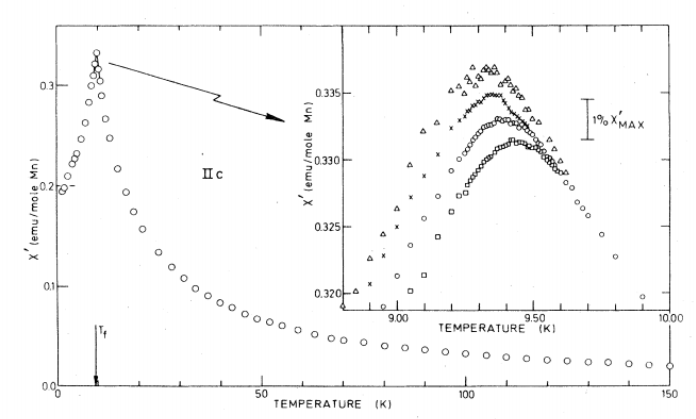
\includegraphics[width=0.6\textwidth]{img/cusp_low_freq.png}}\\  
\subfigure[Susceptibilities of CuMn vs temperature for 1.08\% and 2.02\% Mn.
(Natata et.al 1979)]
{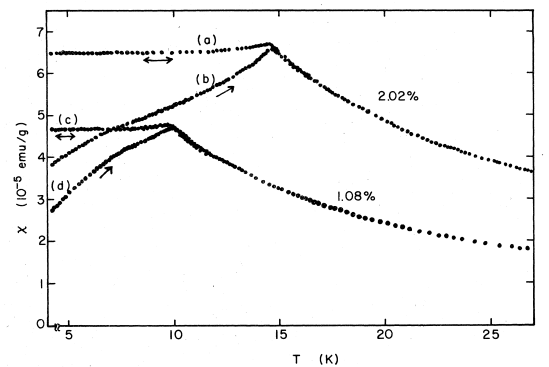
\includegraphics[width=0.6\textwidth]{img/fc_zfc.png}}
  \caption{Magnetic features of spin glass in a small field.}
\end{figure}

\section{Theoretical understanding on spin glass}
A simple model that captures the consequences of disorder is an Ising model 
with quenched randomly disordered couplings, first proposed by Edwards and 
Anderson:
\begin{equation}
  \label{eq:EA}
  H=-\sum_{\langle i,j \rangle}J_{ij}S_iS_j-h\sum_iS_i
\end{equation}
Here $S_i$ is the spin in a $d$-dimensional lattice that can take values $\pm 1$,
$\langle i,j \rangle$ indicates nearest neighbors with the coupling $J_{ij}$ between 
them, and $h$ is the external field.
 
Numerical evidence suggests that the criticality of the three dimensional
spin glass systems are largely independent of the distrubtion of the randomness,
that is they are in the same universality class for different distributions. 
But, the two main paradigmatic cases for the $J_{ij}$ in EA model are:
\begin{itemize}
\item Gaussian distribution of random coupling:
  \begin{equation}
    \label{eq:Jij_Gaussian}
    P(J_{ij})=\frac{1}{\sqrt{2\pi}}\exp^{-J_{ij}^2/2}
  \end{equation}
\item Bimodal ($\pm J$) distribution of random coupling:
  \begin{equation}
    \label{eq:Jij_bimodal}
    P(J_{ij})=\frac{1}{2}[\delta(J_{ij}-1)+\delta(J_{ij}+1)]
  \end{equation}
\end{itemize}

\subsection{Frustration}
\label{sec:frustration}
Frustration naturally present in the Hamiltonian in Eq \ref{eq:EA}, when no spin 
configurations can satisfy all couplings at the same time. 
Figure \ref{fig:frustration} demonstrate two situations where frustrations 
happens. In Fig \ref{fig:frustration_geo}, the two spins on the top and the left
are anti-parallelly aligned due to the anti-ferromagnetic coupling between them,
but there is not an preferred spin direction for the third spin that can satisfy
both the anti-ferromagnetic bonds. In Fig \ref{fig:frustration_quench}, the 
frustration comes from the random distribution of $J_{ij}$. 

\begin{figure}
  \centering
  \subfigure[Geometrical Frustration. Here all couplings are anti-ferromagnetic.]{
    \label{fig:frustration_geo}
    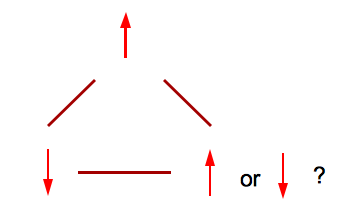
\includegraphics[width=0.4\textwidth]{img/ising-3-spin.png}
  }\hspace{0.5cm}
  \subfigure[Frustration due to randomness. Here $J=-1$ indicates an 
anti-ferromagnetic coupling, while $J=+1$ means ferromagnetic coupling.]{
    \label{fig:frustration_quench}
    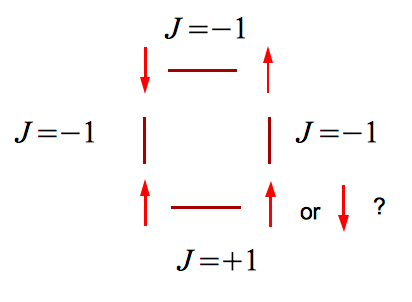
\includegraphics[width=0.4\textwidth]{img/ea-4-spin.png}
  }
  \caption{Frustration in EA model.}
  \label{fig:frustration}
\end{figure}

The frustration is a key factor that leads to many features which make 
spin glass a complex system.
These features include: the existence of many metastable states; the rugged energy 
landscape; and dynamical behaviors such as slow relaxation, irreversibility, 
memory effects, hysteresis, etc. 


\subsection{Pictures on the nature of the spin galss phase}
\label{sec:meanfield-model}

An infinite-ranged version of spin glass models 
was proposed by Sherrington and Kirkpatrick (SK).
\begin{equation}
  \label{eq:SK}
  H=-\frac{1}{\sqrt{N}}\sum_{1\le i\le j\le N}J_{ij}S_iS_j
\end{equation}
Here $J_{ij}$ is chosen from a Gaussian distribution in equation 
\ref{eq:Jij_Gaussian}.
This model has an equilibrium phase transition at $T_c = 1$.
For the spin glass phase below $T_c$, Parisi employed a novel ansatz and 
developed a  possible physical interpretation of the nature of spin glass, 
which is now known as the ``Replica Symmetry Breaking'' (RSB) picture. The main
idea behind the picture is that the spin glass phase consists of an infinite 
number of ``pure states'' that form a hierarchy rather than follow simple symmetry
transformation. 
The ultrametric topology of spin glass states can be represented with a 
genealogical tree. Each end point corresponds to a pure state, and branches 
represent clusters, as sketched in Fig. \ref{fig:TreeRSB}. 

%http://lptms.u-psud.fr/membres/Mezard/Pdf/84_MGSTV_PRL.pdf
%insert tree picture here.

\begin{figure}[!h]
  \label{fig:TreeRSB}
  \centering
  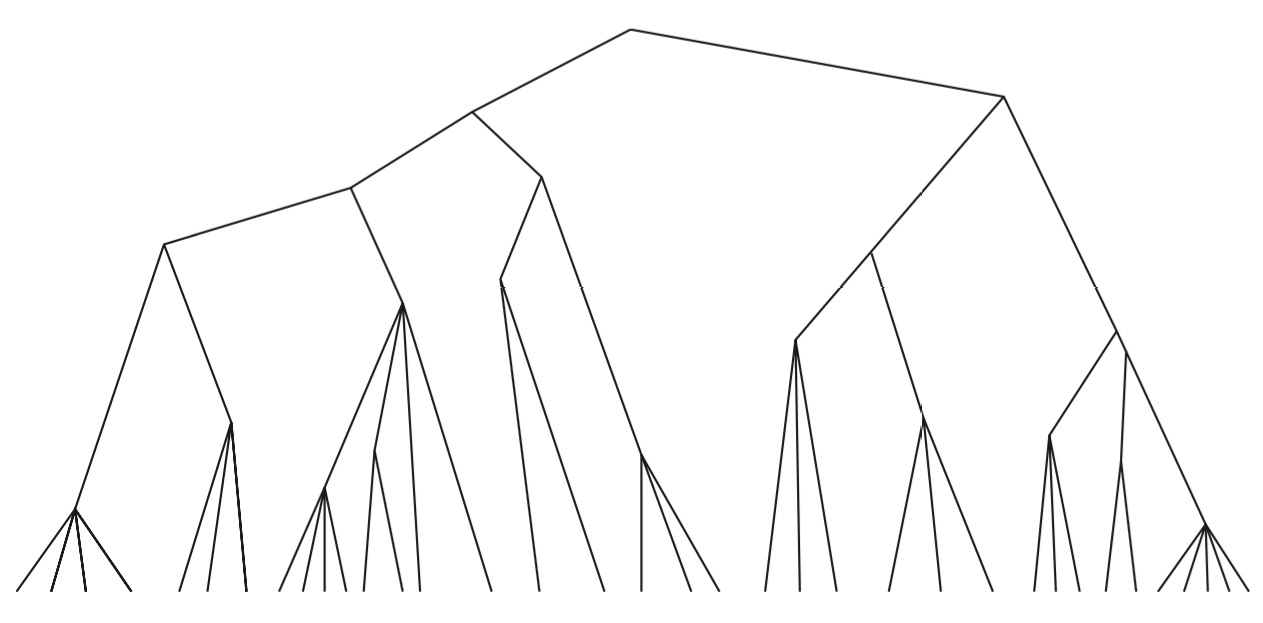
\includegraphics[width=0.6\textwidth]{img/TreeRSB.png}
  \caption{Hierarchical structure of the ensemble of spin-glass states, according
to the RSB picture. The end points represents states; branches (with all their descendents)
represent clusters.}
\end{figure}


RSB is successful in the description of infinite range models, but whether it 
holds in finite dimensions remains the most prominent open question in the study of spin glass systems. 
A competing picture, known as droplet/scaling, is based on domain-wall 
renormalization group ideas. In this picture, there is only a single of
pure states that are spin-flip-symmetrical at low temperature in any finite 
dimension. The difference between the consequence from these two pictures 
will show up in the order paremeters for spin glass as we will define in the following.

%\section{Quantities characterizing spin glass}

The quantity $q$ measures the overlap of the samples after a long time relaxation process. 
It was first studied by the seminal paper by Edwards and Anderson,
\begin{equation}
  \label{eq:q}
  q=\frac{1}{N}\sum_iS_i^\alpha S_i^\beta=\frac{1}{N}\lim_{T\to \infty}\sum_iS_i(t_0)S_i(t_0+T)
\end{equation}
where $\alpha$ and $\beta$ are two copies of lattice with the same disorder 
configuration, but simulated with different random seeds, so they are
statistically independent of each other. The EA order paremeter, q, 
is the order parameter of measuring the breaking of ergodicity. 

The order parameter defined for the spin glass measuring the change of the systems
when the time goes to infinity. In the thermodynamic limit, if this
is zero, the system is ergodic, if this is finite, the system break
the ergodicity. Some parts of the phase space can never be sampled.

In contrast of conventional order parameters which measures the 
spatial pattern, such as magnetization. If the order parameter is non-zero, 
the system is said to undergo spontaneous symmetry breaking, in which the symmetry of 
the states is lower than that of the Hamiltonian. If one calculates
the EA order parameter, said for the ferromagnet, it will
show a finite value. However, this is not a spin glass transition, a
spin glass transition does not comes with a spontaneous symmetry breaking in space.

According to the Parisi solution, for fixed J and (large) N, the structure of 
the overlap is nontrivial, while in droplet picture, in the theromdynamic limit, the distribution is just 
a pair of delta functions at $\pm 1$. 
%insert figure for RSB/droplet overlap here

\begin{figure}
  \centering 
  \subfigure[RSB (mean field) picture]{
    \label{fig:overlap_rsb}
    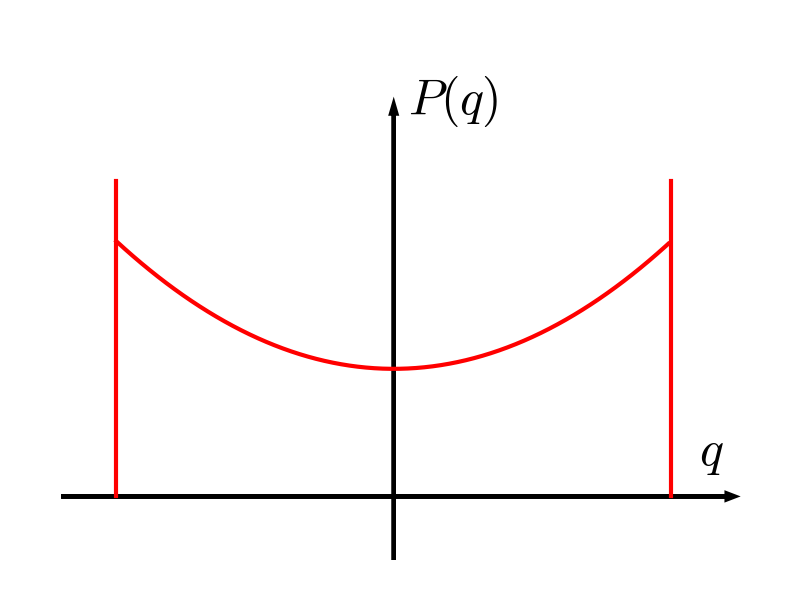
\includegraphics[width=0.4\textwidth]{img/sg/sg_rsb.png}
m  }\hspace{0.5cm}
  \subfigure[Droplet picture]{
    \label{fig:overlap_droplet}
    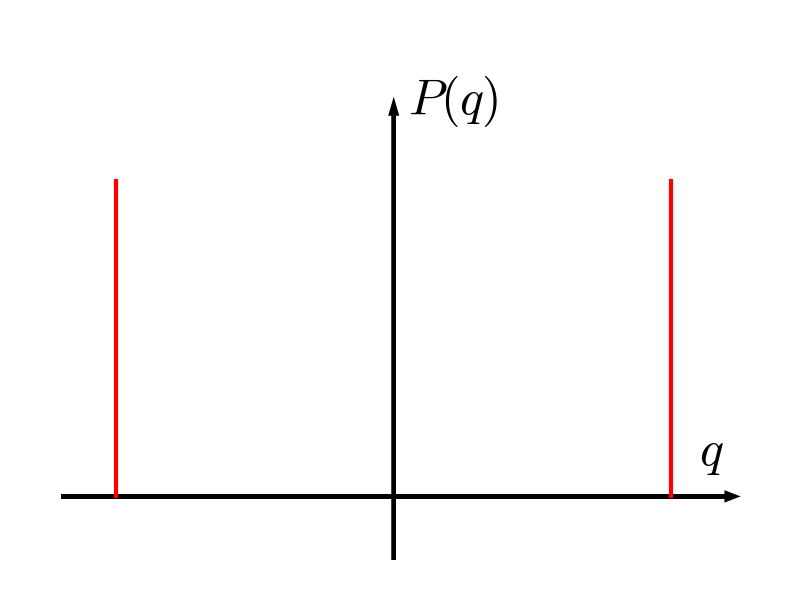
\includegraphics[width=0.4\textwidth]{img/sg/sg_droplet.png}
  }
  \caption{Sketch of the overlap distribution $P(q)$ for the RSB picture, and the
droplet picture.}
  \label{fig:overlap}
\end{figure}


\section{Difficulties and Outstanding Problems}
The EA model is a deceptively simple problem. Since it is a classical spin 
model, one may think that its numerical study can be simply carried out by Monte
Carlo methods on conventional hardware. One of the defining signatures of spin glass 
systems is their long relaxation time. 
For sufficiently low temperatures, the system becomes very sluggish and 
equilibration is prohibitively difficult even for modest systems sizes. 
Moreover, it has been shown that finding the ground state of the three 
dimensional EA model is an NP-hard problem. \cite{Barahona-1982} 
Until recently, there has been no consensus on whether there is a finite spin 
glass critical temperature in the three dimensional EA model.

%It also requires a large number of disorder realizations to reach any 
%meaningful result.

Due to the difficulty in the simulation, there is still no general consensus on
which of the two competing pictures is correct. 
An import discriminator between the theories is the predicted behavior of 
the system when the temperature is decreased in the presence of an applied magnetic
field. 
In the mean field approximation, the de Almeida-Thouless line separates the 
high-temperature paramagnetic phase from the spin glass phase (Fig.\ref{fig:at_rsb}). 
With the droplet/scaling theory, an applied magnetic field is predicted to remove
the phase transition completely (Fig.\ref{fig:at_droplet}).

\begin{figure}
  \centering
  \subfigure[RSB (mean field) picture]{
    \label{fig:at_rsb}
    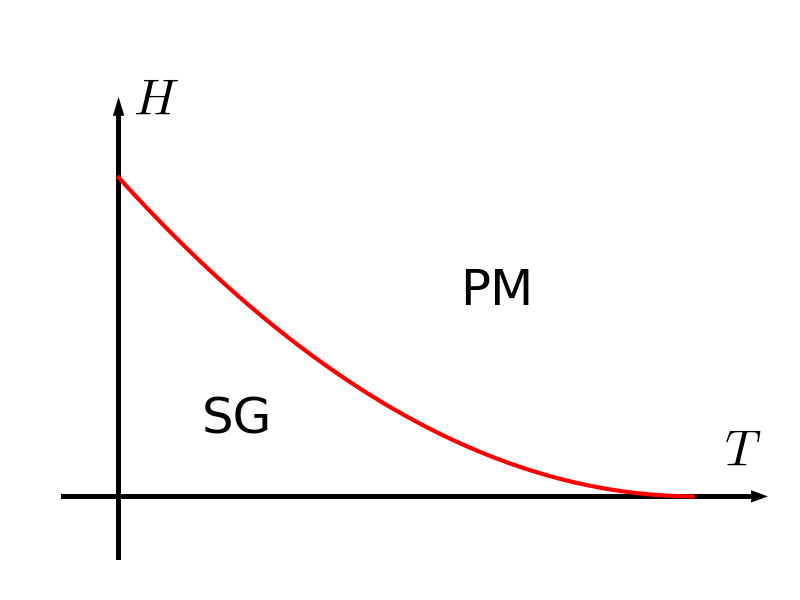
\includegraphics[width=0.4\textwidth]{img/sg/at_rsb.png}
  }\hspace{0.5cm}
  \subfigure[Droplet picture]{
    \label{fig:at_droplet}
    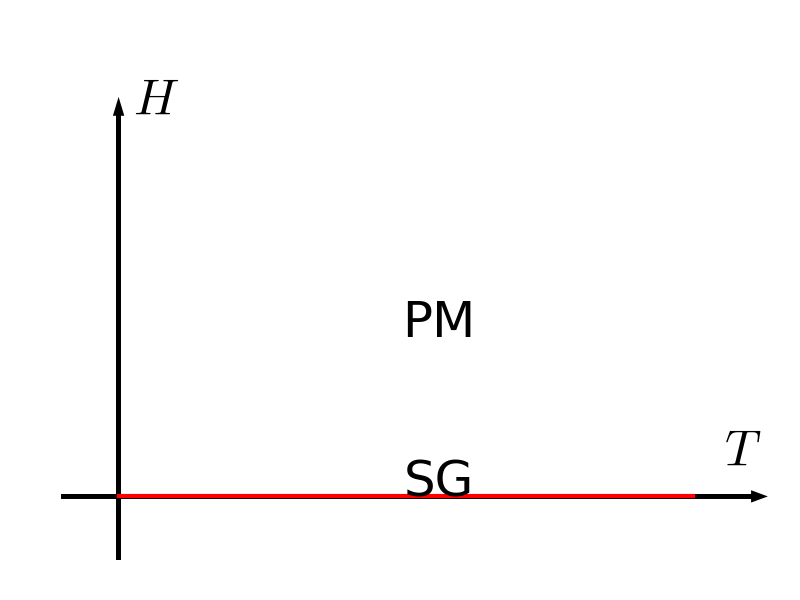
\includegraphics[width=0.4\textwidth]{img/sg/at_droplet.png}
  }
  \caption{Sketch of the AT line in the RSB picture, and the droplet picture.}
  \label{fig:at_line}
\end{figure}

Recent work supports that there is only a pair of two ground states in two dimensions.
In four dimensions, the JANUS show evidence for the presence of a spin glass
phase transition in a field. In three dimensions, numerical simulations give 
conflicting results.


\section{Algorithms for spin glass simulation}
The breakthrough in the numerical study of spin glass systems came with the 
introduction of the parallel tempering method. Parallel tempering (PT), also known
as replica exchange, is a simulation method aimed at improving the dynamic 
properties of Monte Carlo sampling. Instead of simulating one Markov chain at 
a time, one runs N copies of the system with random seeds at different 
temperatures, and exchange configurations based on the detailed balance condition.
By making the configurations at high temperatures available to simulations at 
low temperatures, this method allows better sampling over the entire energy
landscape. We discuss this method further in \ref{sec:PT}.

Simulated annealing (SA) is another commonly used algorithm for heuristic optimization,
due to its simplicity and effectiveness. In physics, one usually select the 
energy as the cost function, start the Monte Carlo simulation at a high temperature
and slowly tune down the temperature during the simulation, and in the end the
configuration of the system would stay in a local minimum. With slow-enough annealing
and multiple repetitions, one would expect to find the global minimum.  

Population annealing (PA) combines simulated annealing and Boltzmann weighted 
differential reproduction within a population of replicas to sample equilibrium 
states. Similar to simulated annealing, population annealing involves lowering 
the temperature of the system at a sequence of temperatures. However, PA uses a 
population of replicas and this population is resampled at each time step.
By doing this, PA aims to ensure that the population always stay close to the 
Gibbs distribution. Population annealing is naturally a massively
parallel algorithm, as realistic spin glass simulation using population 
annealing require population sizes of the order $10^6$ or more.
%http://arxiv.org/pdf/1508.05647v2.pdf

Another possibly to overcome the diverging autocorrelation time problem is the 
multicanonical reweighting method. Instead of sampling the the Boltzmann 
distribution $P=\exp(-\beta Ep)$, multicanonical ensemble uses the 
Metropolis–Hastings algorithm with a sampling distribution given by the inverse 
of the density of states of the system. The density of states has to be known 
a priori, or be computed using techniques such as the Wang and Landau algorithm.



% \section{Computer simulations review}
% Universality in three-dimensional Ising spin glasses: A Monte Carlo study
% arXiv:cond-mat/0602212 Phys. Rev. B, 73, 224432 (2006)


% 20. H. G. Katzgraber and A. P. Young, “Monte Carlo studies of the one-dimensional Ising spin glass with power-law interactions,” Phys, Rev. B, vol. 67, p. 134410, 2003. (cond-mat/0210451).
% 21. H. G. Ballesteros et al., “Critical behavior of the three-dimensional Ising spin glass,” Phys. Rev. B, vol. 62, p. 14237, 2000. (cond-mat/0006211).
% 22. E. Marinari, G. Parisi, and J. J. Ruiz-Lorenzo, “On the phase structure of the 3d Edwards Anderson spin glass,” Phys. Rev. B, vol. 58, p. 14852, 1998.
% 23. H. G. Katzgraber and A. P. Young, “Absence of an Almeida-Thouless line in three-dimensional spin glasses,” Phys. Rev. Lett., vol. 93, p. 207203, 2004. (cond- mat/0407031).

%%% Local Variables:
%%% mode: latex
%%% TeX-master: "../thesis"
%%% End:
